\documentclass[main.tex]{subfiles} % Subfile-Class


% ============================================================================== %
%                            Subfile document                                    %
% ============================================================================== %

\begin{document}

% Template

\subsubsection{Schnittstelle Raspberry Pi}
Wie Eingangs im Abschnitt~\ref{sec:Gesamtuebersicht_Elektro} erwähnt, wird die
Steuerungseinheit, der Raspberry Pi, mit einer eigens entwickelten Leiterplatte
in das Gesamtsystem eingebunden.

Diese erfüllt die folgenden Aufgaben

\begin{description}
      \item[Digitale Ein- \& Ausgänge] Im Hinblick auf die digitale Ein- und
            Ausgangs-Funktionalität der Leiterplatte ist festzustellen, dass diese über
            vier digitale Eingänge verfügt, die auf einem Spannungspegel von 12 V arbeiten.
            Zwei digitale Ausgänge sind in der Lage, auch grössere Lasten bis zu 3 A zu
            schalten, wobei hier auf den Energiebedarf des Gesamtsystems geachtet werden
            muss.
      \item[Schnittstellen Schalter] Im Hinblick auf die Schnittstellen ist festzuhalten,
            dass sowohl ein Wahlschalter als auch ein Starttaster mit dem Raspberry Pi
            verbunden werden können. Der Starttaster wird mit einem Komparator und einem
            RC-Filter bereits in Hardware entprellt.
      \item[Schnittstelle Kommunikation] Die Schnittstelle zur Kommunikation wird durch den
            UART-Kanal des Raspberry Pis mit einer RS422-Schnittstelle zur Kommunikation
            mit dem Gesamtsystem aufbereitet.
      \item[Sensorschnittstellen] Darüber hinaus können über die $I^2C$-Schnittstellen
            einfache Sensoren angeschlossen werden. Es sind sowohl Schnittstellen für 5V
            und 3.3V Logikpegel vorhanden, was die Leiterplatte sehr vielseitig einsetzbar
            macht.
      \item[Spannungsversorgung] Im Hinblick auf die Spannungsversorgung wird die
            12-Volt-Versorgungsspannung mit einem 5-Volt-3-Ampere-DCDC-Steller und LDO für
            den Raspberry Pi aufbereitet und gefiltert.
      \item[Sonstige Besonderheiten] Darüber hinaus bietet die RaspberryHAT-Leiterplatte
            einige optische Anzeigeelemente, die zu Debugzwecken einfache digitale Signale
            optisch darstellen können. Daneben ist das Board mit einem Piezo Summer
            ausgestattet, welcher die akustische Signalisierung von Betriebszuständen, wie
            z.B. das Erreichen eines Zielpunkts zulässt.
\end{description}

Die Abbildungen~\ref{fig:RaspberryHAT_draufsicht} und
~\ref{fig:RaspberryHAT_3D} zeigen das RaspberryHAT - PCB in einer Draufsicht
und in einer 3D-Ansicht. In Abbildung~\label{fig:RaspberryHAT_3D} ist
ersichtlich, wie der Raspberry Pi an dieses Board angeschlossen wird.

\begin{figure}[H]
      \centering
      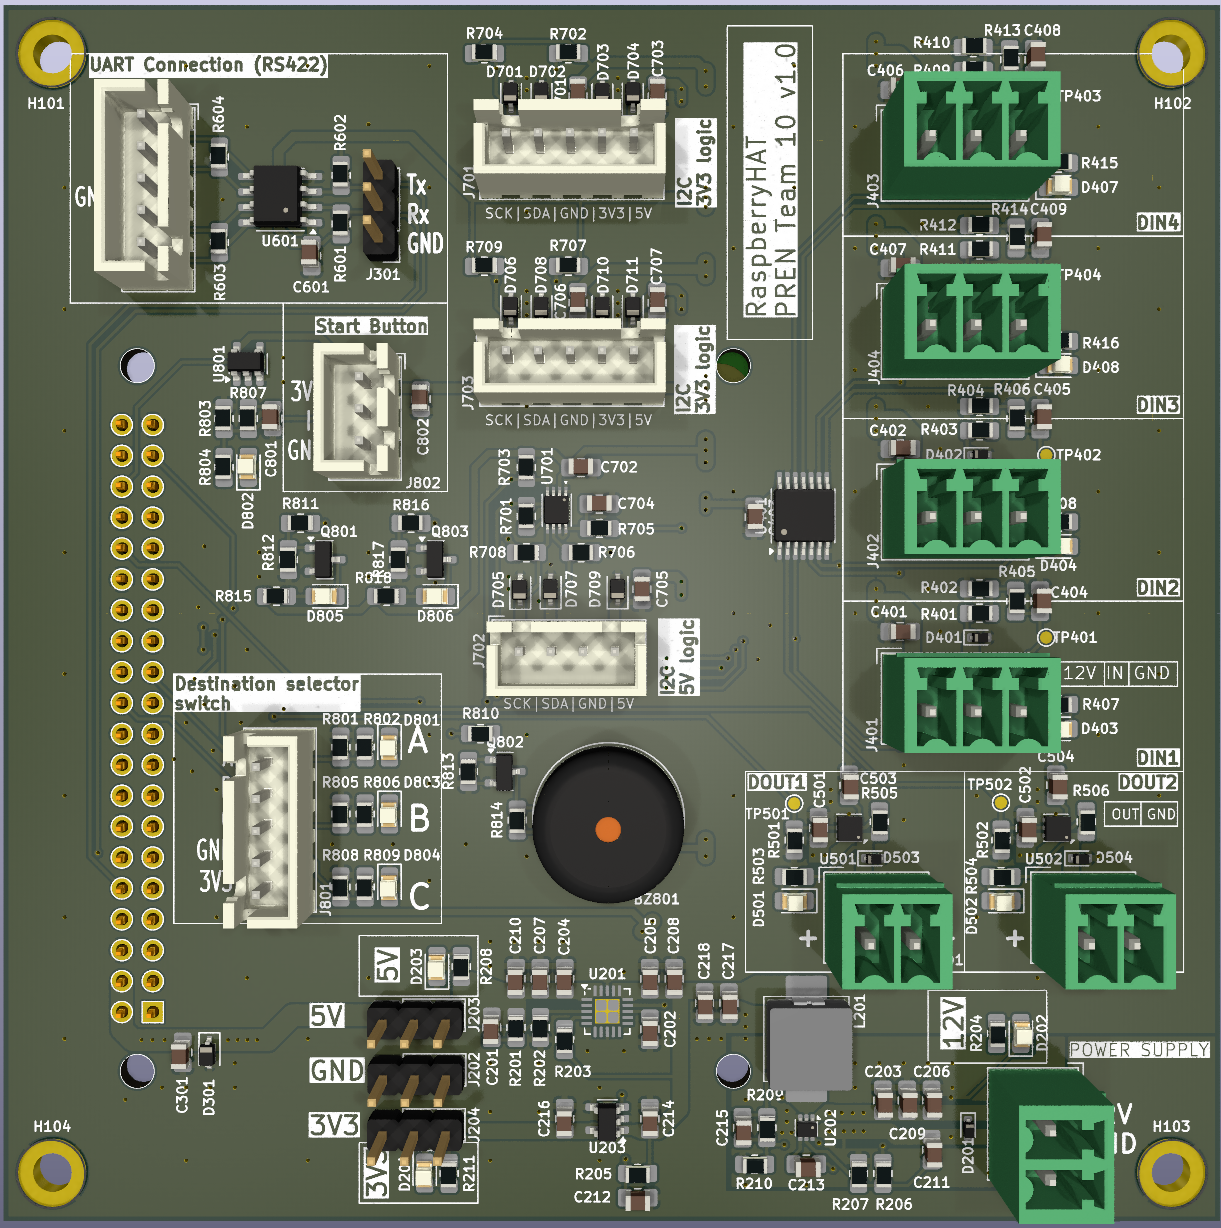
\includegraphics[width=0.75\textwidth]{./fig_RaspberryHAT/RaspberryHAT_draufsicht.png}
      \caption{RaspberryHAT in Draufsicht}~\label{fig:RaspberryHAT_draufsicht}
\end{figure}

\begin{figure}[H]
      \centering
      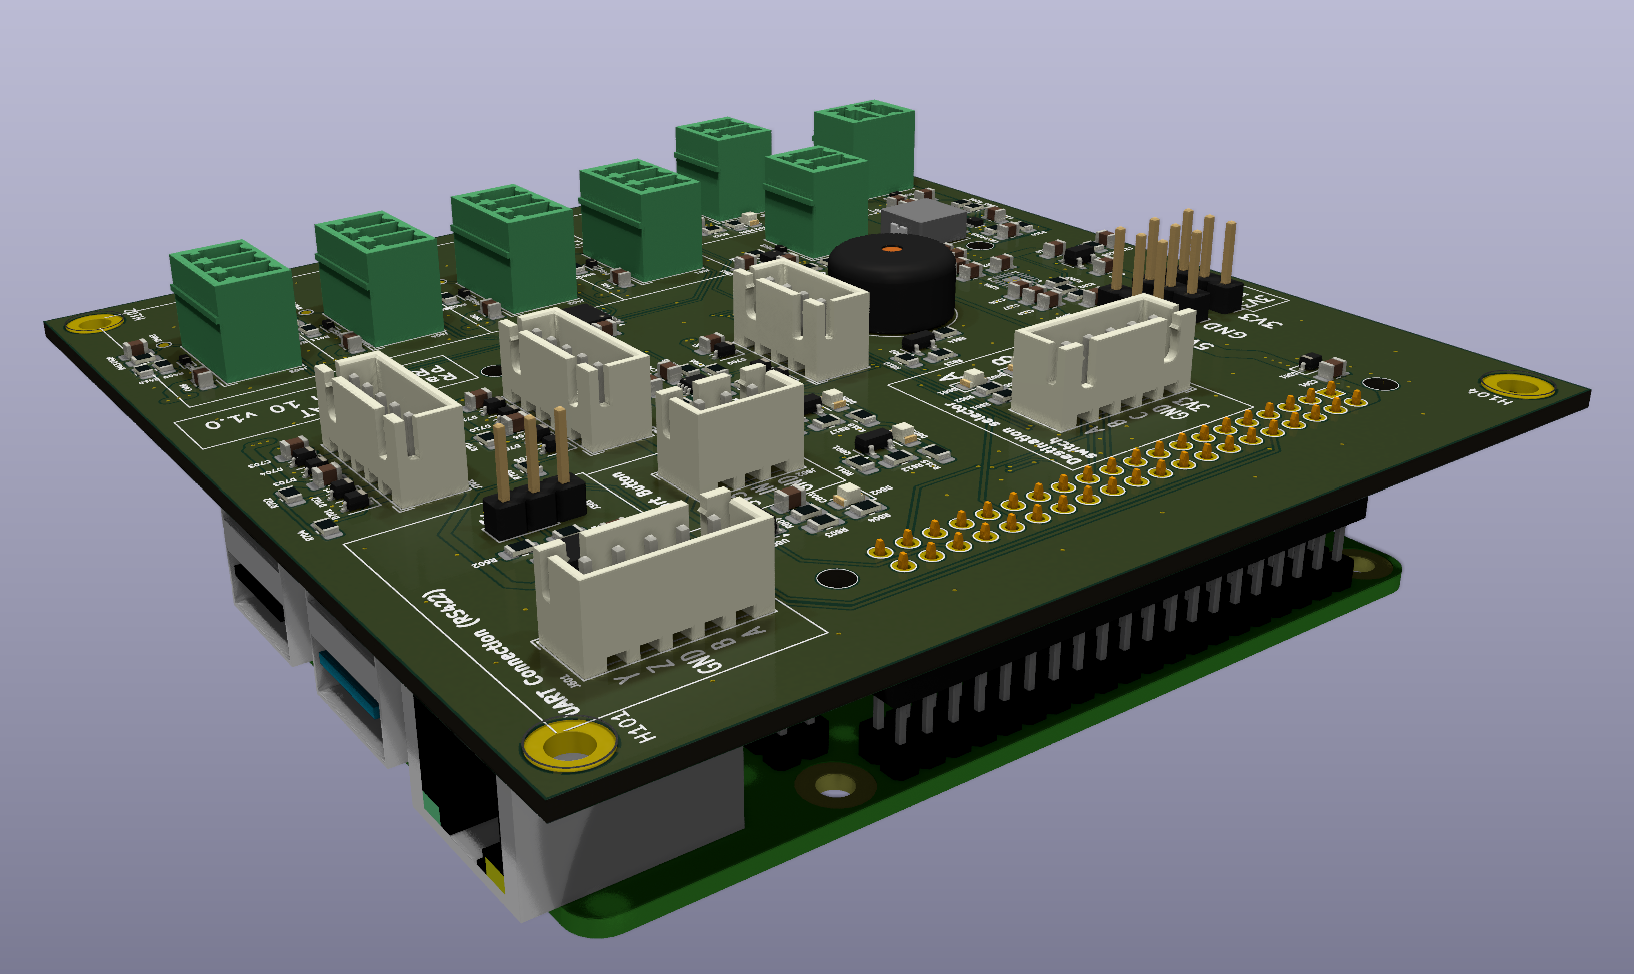
\includegraphics[width=0.75\textwidth]{./fig_RaspberryHAT/RaspberryHAT_3D.png}
      \caption{RaspberryHAT in 3D Ansicht}~\label{fig:RaspberryHAT_3D}
\end{figure}

Bei der Entwicklung dieser Leiterplatte ist zum grössten Teil auf
Teilbaugruppen des Motioncontrollers sowie des Gripcontrollers zurückgegriffen
worden. Aus Gründen der Übersichtlichkeit ist deshalb auf eine separate
Schaltungsdimensionierung und -beschreibung verzichtet. Die entsprechenden
Designfiles befinden sich nichtsdestotrotz im digitalen Anhang.

\end{document}
